% The \phantomsection command is needed to create a link to a place in the document that is not a
% figure, equation, table, section, section, chapter, etc.
%
% When do I need to invoke \phantomsection?
% https://tex.stackexchange.com/questions/44088/when-do-i-need-to-invoke-phantomsection
\phantomsection


% Multiple-language document - babel - selectlanguage vs begin/end{otherlanguage}
% https://tex.stackexchange.com/questions/36526/multiple-language-document-babel-selectlanguage-vs-begin-endotherlanguage

\chapter[\lang{Basic concepts and the Proposed measure}{Conceitos básicos e a Medida proposta}]
{
    \lang
    {Basic concepts and the Proposed measure}
    {Conceitos básicos e a Medida proposta}
}\label{sec:proposed_measure}

    \begin{flushright}
         
    \end{flushright}

Stops and moves by definition are different and heterogeneous trajectory elements. A stop may have a spatial position, a start and end time, a category, or a set of attributes related to the category (e.g. Category hotel, stars, rate, price), etc. A move always starts and ends in a stop and may be characterized by different attributes as average speed, traveled distance, sequence of streets, duration, the sequence of raw points, etc. These attributes are defined according to the needs of the application. 

In order to deal with these heterogeneous elements (stops and moves), we introduce the concept of \emph{movement element}. A movement element is a new representation that is not treated by other measures, mainly MSM, which supports only stops. Indeed, MSM does not consider the order of trajectory elements, while in our approach we preserve the sequence of both stops and moves in a movement element.

\begin{definition}[Movement element]
\label{def:movement_element}
A movement element e = \emph{(stopS, move, stopE)} is a tuple formed by a start stop \emph{stopS}, the move between \emph{stopS} and \emph{stopE}, and the end stop \emph{stopE}, where \emph{stopS} and \emph{stopE} are two consecutive stops.
\end{definition}


Hereafter we will consider a semantic trajectory as a sequence of \textit{movement elements}, as follows: 
$P=\langle e_1 = (s_1,m_1,s_2), e_2$\newline $= (s_2,m_2,s_3), ..., e_n = (s_n,m_n,s_{n+1}) \rangle$.

Notice that we define a movement element as a trajectory part, and this structure will be used for the proposed similarity measure, where one trajectory will be compared with another one based on their movement elements.



We analyze the similarity of a movement element $a\in A$ with another movement element $b\in B$, where A and B are semantic trajectories, in two parts: their stops and their moves. The basis for measuring the similarity of these two parts is the \emph{match} function, given in Equation \ref{func:match1}. The function returns 1 if the distance between an attribute (also called dimension) of two movement elements is less than a given threshold \emph{maxDist}, and zero otherwise. This function is used for measuring the distance of all dimensions of both: the stops and the moves.

\begin{equation}
%\scriptsize
\label{func:match1}
  match_i(a, b) = 
  \begin{cases} 
      1 & dist_i(a, b) \leq maxDist_i \\
      0 & otherwise
  \end{cases}
\end{equation}

To compute a total score for two movement elements $a$ and $b$ we define the function \emph{score(a,b)} in Equation \ref{func:score1}, where, $w_{stop}$ and $w_{move}$ are the weights of the stops and the moves, respectively, and their sum should be one. The importance of either stops or moves can vary from one application to another, so we can use the weights to give the respective importance. 


\begin{equation}
%\scriptsize
\label{func:score1}
score(a, b) = scoreStop(a, b) * w_{stop} + scoreMove(a, b) * w_{move}  
\end{equation}


In our measure we consider a score for the stops (scoreStop) and a score for the move (scoreMove). The functions \emph{scoreStop(a,b)} and \emph{scoreMove(a,b)} are defined in Equations \ref{func:scoreStop1} and \ref{func:scoreMove2}, respectively. In both equations, $r$ and $q$ are the number of dimensions (attributes) of stops and moves, respectively. The score of the stops, computed according to Equation \ref{func:scoreStop1}, is given by the average of all dimension matches of the start and end stops of two movement elements $a$ and $b$. 


\begin{equation}
%\scriptsize
\label{func:scoreStop1}
\begin{split}
  scoreStop(a, b) = \sum\limits_{i=1}^r & (match_i(a_{stopS}, b_{stopS}) + \\
  &  match_i(a_{stopE}, b_{stopE}))\div 2* w_{i}
\end{split}
\end{equation}


\begin{equation}
%\scriptsize
\label{func:scoreMove2}
\begin{split}
scoreMove(a, b)  & = 
  \begin{cases} 
      \sum\limits_{i=1}^q match_i(a_{move}, b_{move}) * w_{i} & if matchStops(a, b)\\
      0 & otherwise
  \end{cases}
\end{split}
\end{equation}


%The sum of the weights in Equations \ref{func:scoreStop1} and \ref{func:scoreMove2} should be one.
Note in Equation \ref{func:scoreMove2} that the \emph{scoreMove} depends on the function \textit{matchStops(a, b)}. {The intuition is that two moves should be evaluated only if their starting positions (starting stops) are spatially close and the ending positions (ending stops) are close as well.}
The function \emph{matchStops(a,b)} is true when the {spatial distance} between $a_{stopS}$ and $b_{stopS}$  as well as between $a_{stopE}$ and $b_{stopE}$ is less than or equal to $maxDist$.
    
    %\textcolor{red}{In real scenarios, this means that if we want to analyze movement elements, for instance, from France to Italy, we do not need to compare these trajectories with others moving from France to Spain, since the ending stop is different}.

{Figure {\ref{fig:move}} shows an example of four movement elements representing part of four trajectories. The movement elements are $e_1=<A, P_1, B>$, $e_2=<A, P_2, B>$, $e_3=<A, P_3, B>$ and $e_4=<A, P_4, C>$, where $A$, $B$, and $C$ are the stops, and $P_i$ are the moves. Considering $e_1$ and $e_4$, the function $match(P_1,P_4)$ will be executed only if the function $matchStops(B,C)$ is true, i.e., $dist(B,C) \leq  maxDist$. If $dist(B,C) > maxDist$, the value of $scoreMove(e_1,e_4)$ is zero.
%So the \emph{moves} of the movement elements $<A, P_1, B>$, $<A, P_2, B>$, $<A, P_3, B>$ will be analyzed because they have the same start and end stop.}
}

 %and three trajectories move to $B$ following three different paths.  In the example in Figure \ref{fig:move}, if we are interested in trajectories moving from A to B, our measure will only analyze the moves $P1$, $P2$, and $P3$ of trajectories going from A to B, and these three moves will not be compared with $P4$. 

%{Differences among the three movement elements rely exclusively on the differences of the move. On the other hand, the difference of these movement elements to movement element $<A, P_4, C>$ is more evident, since if it end stop is distinct, the move is distinct too. Based on this, SMSM do not compare the move of $<A, P_4, C>$ with the others movement element.}

{The function \emph{scoreMove()} guarantees a partial order in the similarity analysis. %, what has not been considered by MSM, which is the closest measure to our approach, but that considers only stops and without any order. Considering that the four movement elements in Figure {\ref{fig:move}} belong to four different trajectories, MSM would give the same similarity for the parts of the trajectories going from $A$ to $B$, because it does not look the moves, and 50\% similarity with the trajectory going from $A$ to $C$ because they share 50\% of the stops.
Suppose the example in  Figure {\ref{fig:move}} is a real scenario, where $A$, $B$, and $C$ represent  places as France, Italy, and Spain, respectively. We believe that the three trajectories going from France ($A$) to Italy ($B$) must have their move analyzed because they visit the same sequence of places, while the trajectory that goes from France ($A$) to Spain ($C$) does not share the same destination, so the move of this trajectory is not compared with the others, and the function $scoreMove()$ has values zero.}



\begin{figure}[h]
\centering
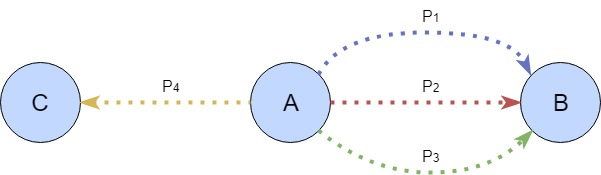
\includegraphics[width=0.75\textwidth]{Images/Toy_trajectories.jpg}
\caption{\label{fig:move} Movement elements: stop $A$ to stop $B$ with the moves $P_1$, $P_2$, and $P_3$; and Movement element: $A$ to $C$ with the move $P_4$}
\end{figure}

Having defined the score for stops and moves for comparing movement elements, Equation \ref{func:parity} defines the parity of two semantic trajectories $A$ and $B$. The parity of $A$ with $B$ is the sum of the highest score of all the elements $a \in A$ when compared with all the elements of $B$.
\begin{equation}
\label{func:parity}
parity(A, B) = \sum\limits_{a\in A} \textbf{max}\{\textit{score}(a, b) : b \in B\}
\end{equation}

Finally, we can define the global similarity of two trajectories $A$ and $B$ with $SMSM$. Equation \ref{func:SMSM1} defines the stops and moves similarity measure $SMSM(A,B)$ by the average parity of $A$ with $B$ and of $B$ with $A$. {The average parity is given by the sum of both parities over the sum of the number of elements in $A$ ($|A|$) and the number of elements in $B$ ($|B|$).}

\begin{equation}
\label{func:SMSM1}
%\scriptsize
\begin{split}
  SMSM(A, B) = 
  \begin{cases} 
      0 & if  |A| = 0 \vee |B| = 0 \\
      \frac{parity(A, B) + parity(B, A)}{|A| + |B|} & otherwise
  \end{cases}
\end{split}
\end{equation}



\section{Evaluation over a running example}

In this section we present a running example, comparing SMSM and MSM, since MSM is the closest approach.
Let us consider the two trajectories shown in Figure \ref{fig:bus}. Trajectory $Q$ represents the daily routine of a professor, that starts his day at the gym in the morning, while trajectory $P$ is the daily routine of a student, that starts his day at a coffee shop. Both trajectories visit the same places, sharing some streets, but in totally different order. The trajectories are annotated with the stop category, start and end time of the stop, an hypothetical geographic position ($x, y$) of the stop and the main street followed during the moves. So considering the {notation \textit{stop name ((x, y), [start timestamp - end timestamp])}}, the student has the following movement behavior: stays at \textit{Home} (\textit{(96,215)}, [\textit{8pm-8am}]), {then} he goes via Edu Vieira street to have breakfast at the \textit{Coffee shop} (\textit{(182,201)}, [\textit{8:50am-10am}]), and from there goes via Delfino Conti street to the \textit{University} (\textit{(59,127)}, [\textit{10:25am-6:10pm}]), finishing the day moving via Henrique Fontes street to the \textit{Gym} (\textit{(268,63)}, [\textit{7:30pm-9pm}]). The professor (trajectory $Q$) goes from \textit{Home} (\textit{(13,81)}, [\textit{7pm-7am}]) via Beira-mar avenue for jogging at the \textit{Gym} (\textit{(268,63)}, [\textit{7:30am-8:30am}]). After he goes to the \textit{Coffee shop} (\textit{(182,201)}, [\textit{8:45am-9:55am}]) via Edu Vieira street, and via Delfino Conti reaches the \textit{University} (\textit{(59,127)}, [\textit{10:15am-7:45pm}]) to teach his classes until the end of the day. We have two trajectories $P$ and $Q$ with their stops and moves annotated with the category of the place, the spatial position of the visited place, the time of the visit, and the name of the street to represent the move.
\begin{figure}[h!]
\centering
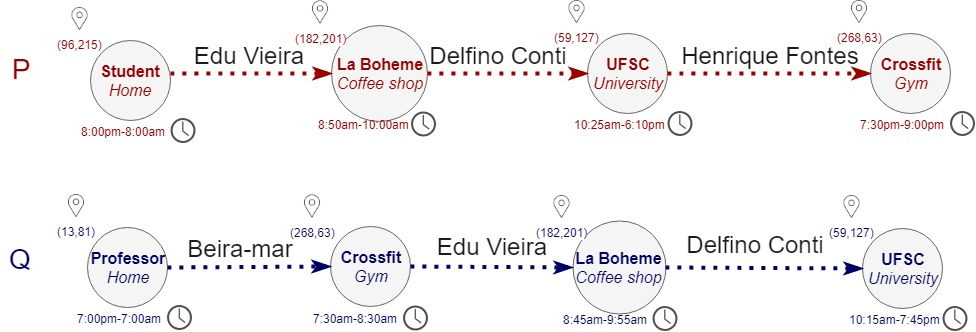
\includegraphics[width=1\textwidth]{Images/running_example.jpg}
\caption{\label{fig:bus} Semantic Trajectories $P$ (Student) and $Q$ (Professor) with stops and moves}
\end{figure}


In order to calculate the SMSM similarity value, we first need to construct all movement elements for each trajectory. Table \ref{tab:SMSM_tuples} lists these elements, where each element contains the start stop, the name of the street followed during the move, and the next stop. 

\begin{table}[h!]
\scriptsize
  \centering
 \resizebox{\linewidth}{!}{%
  \begin{tabular}{|c|c|}
  	\hline
		\textcolor{Red}{\textbf{Student (P)}} & \textcolor{Blue}{\textbf{Professor (Q)}}\\
  	\hline
      $<$Home, Edu Vieira, Coffee shop$>$&$<$Home, Beira-mar, Gym$>$\\
      $<$Coffee shop, Delfino Conti, University$>$&$<$Gym, Edu Vieira, Coffee shop$>$\\
      $<$University, Henrique Fontes, Gym$>$&$<$Coffee shop, Delfino Conti, University$>$\\
  	\hline
  \end{tabular}
  }
  \caption{Movement elements}
  \label{tab:SMSM_tuples}
\end{table}

To measure the distance between two movement elements, in this example we use the following distance functions for each stop dimension:
\begin{itemize}
  \item Space: the Euclidean distance between the centroids of the stops;
      \item  Time:  {let $[t1, t2]$ be the time interval of a stop. The time distance of two stops is given by:}
\begin{equation} \label{func:time_interval}
	dist_t(a, b) = 1 - \dfrac{duration([a.t1, a.t2] \cap [b.t1, b.t2])}{duration([min(a.t1, b.t1), max(a.t2, b.t2)])}
\end{equation}
{We use this formula in order to have a proportion of the time intersection and not an absolute value.}
  \item Semantics: the distance is equal to 0 in case of exact match and equal to 1 otherwise.
\end{itemize}

For the sake of simplicity, for the move, in this example we consider only the semantic information, i.e., the name of the followed street, where the distance is equal to 0 in case of exact match of street name and equal to 1 otherwise.
We consider that stops and moves have the same weight and also the dimensions space, time and semantics of the stops.

In this running example we use as thresholds \textit{maxDist\textsubscript{space}} = 100  and \textit{maxDist\textsubscript{time}} = 0.5, i.e. two stops are said as matched in time when both share half of their period in that stop.
With distance functions and threshold values defined and elements constructed, we use Equation \ref{func:score1} to measure the similarity values between all element dimensions, computing first the match in both start and end stops and if the stops match we compute the match for the move. 

To better understand how to measure the movement element similarity let us consider  the following two movement elements: 
\begin{itemize}

\item $element_{P}= \\ \ <Home_{[8pm-8am]}, Edu Vieira,$ $Coffee\ shop_{[8:50am-10am]}>$
\item $element_{Q}= \\ \ <Home_{[7pm-7am]}, Beira-mar, Gym_{[7:30am-8:30am]}>$ 
\end{itemize}
First, we apply the function $match()$ (Equation \ref{func:match1}) for the stops. In this case, the start stops have some degree of similarity: their semantics is the same and the time distance of $Home_{P}$ and $Home_{Q}$ is $\approx 0.15$, lower than our defined threshold of $0.5$. However, the spatial distance is $dist_{eucl}(Home_{P}, Home_{Q}) \approx 158 $, higher than the defined threshold (100), so not matching in space, only in time and semantics, leading to a similarity score of $2/3$ between start stops $Home_{[8pm-8am]}$ and $Home_{[7pm-7am]}$. The end stops (Gym and Coffee Shop) are dissimilar in space (with a distance of $\approx 163$), in time (no overlap), and in semantics, then the similarity score between both end stops is $0.0$.

 Equation \ref{func:scoreStop1} computes the stops similarity as the average similarity of start stops  and end stops as: $scoreStops($$element_{P}$, $element_{Q}$) = $(2/3 + 0) / 2 \approx 0.33$.
 As the function $matchStops()$ is false in this example since $dist_{eucl}(Coffee$ $shop_{P}, Gym_{Q}) > 100$, when applying Equation \ref{func:scoreMove2}, the function
$scoreMove()=0$. Then, Equation \ref{func:score1} computes the movement element similarity as the sum of stops similarity weighted by $w_{stops}$ and the move similarity weighted by $w_{move}$. In this example, $score($$element_{P}$, $element_{Q}$) = $(0.33 * 0.50) + (0.00 * 0.50) \approx 0.17$. Table \ref{tab:SMSM_scores} summarizes SMSM similarity scores between all movement elements.

\begin{table}[h]
\scriptsize
  \centering
 \resizebox{\linewidth}{!}{%
  \begin{tabular}{|l|c|c|c|}
  	\hline
		\backslashbox[48mm]{Q}{P}& 
        \makecell{$<$\textcolor{RawSienna}{\textbf{Home}}, Edu V., \textcolor{OliveGreen}{\textbf{Coffee}}$>$ \\ \textcolor{RawSienna}{$[$8pm-8am$]$~~\textcolor{OliveGreen}{$[$8:50am-10am$]$}} \\ \textcolor{RawSienna}{(96,215)}~~~~~~~~~~~\textcolor{OliveGreen}{(182,201)}} & 
        \makecell{$<$\textcolor{OliveGreen}{\textbf{Coffee}}, Delfino C., \textcolor{Mahogany}{\textbf{University}}$>$ \\ \textcolor{OliveGreen}{$[$8:50am-10am$]$}~~\textcolor{Mahogany}{$[$10:25am-6:10pm$]$} \\ \textcolor{OliveGreen}{(182,201)}~~~~~~~~~~~~~~~~~~~\textcolor{Mahogany}{(59,127)}} & 
        \makecell{$<$\textcolor{Mahogany}{\textbf{University}}, Henrique F., \textcolor{Fuchsia}{\textbf{Gym}}$>$ \\ \textcolor{Mahogany}{$[$10:25am-6:10pm$]$}~~\textcolor{Fuchsia}{$[$7:30pm-9pm$]$} \\ \textcolor{Mahogany}{(59,127)}~~~~~~~~~~~~~~~~~~~~\textcolor{Fuchsia}{(268,63)}}\\
  	\hline
      \makecell{$<$\textcolor{RawSienna}{\textbf{Home}}, Beira-mar, \textcolor{Fuchsia}{\textbf{Gym}}$>$\\ \textcolor{RawSienna}{$[$7pm-7am$]$}~~\textcolor{Fuchsia}{$[$7:30am-8:30am$]$} \\ \textcolor{RawSienna}{(13,81)}~~~~~~~~~~~~~~~\textcolor{Fuchsia}{(268,63)}}
      				&0.17&0&0.25\\
      \makecell{$<$\textcolor{Fuchsia}{\textbf{Gym}}, Edu V., \textcolor{OliveGreen}{\textbf{Coffee}}$>$\\ \textcolor{Fuchsia}{$[$7:30am-8:30am$]$}~~\textcolor{OliveGreen}{$[$8:45am-9:55pm$]$} \\ \textcolor{Fuchsia}{(268,63)}~~~~~~~~~~~~\textcolor{OliveGreen}{(182,201)}}
      				&0.25&0&0\\
      \makecell{$<$\textcolor{OliveGreen}{\textbf{Coffee}}, Delfino C., \textcolor{Mahogany}{\textbf{University}}$>$\\ \textcolor{OliveGreen}{$[$8:45am-9:55am$]$}~~\textcolor{Mahogany}{$[$10:15am-7:45pm$]$} \\ \textcolor{OliveGreen}{(182,201)}~~~~~~~~~~~~~~~~~~\textcolor{Mahogany}{(59,127)}}
      				&0.08&1&0\\
  	\hline
  \end{tabular}
  }
  \caption{Similarity scores for SMSM}
  \label{tab:SMSM_scores}
\end{table}

After  computing the similarity scores of both trajectories, with Equation \ref{func:parity} we compute the parity of trajectories, summing the highest scores of all movement elements of one trajectory when compared with all elements of the other trajectory. The parity calculus of $parity(P, Q) = (0.25 + 1.00 + 0.25) = 1.50$ and $parity(Q, P) = (0.25 + 0.25 + 1.00) = 1.50$.
The final SMSM score is given by Equation \ref{func:SMSM1} with $(parity(P, Q) + parity(Q, P)) / (|P| + |Q|) = (1.50 + 1.50) / (3 + 3) = 0.50$, indicating that the trajectories have some degree of similarity, since the two trajectories have several common stops at similar time, move across the same streets, but the most important is that the order of the stops is different. Notice from Table \ref{tab:SMSM_scores} that movement elements where either the start stops or the end stops match, still have a degree of similarity, which is the case of the movement elements $<Home, Edu Vieira, Coffee shop>$ and $<Home, Beira-mar, Gym>$.

{To compare SMSM with MSM, which is the closest work to our approach, we used for MSM the same thresholds for the stops and the same weights for space, time and semantics.}
%use as thresholds \textit{maxDist\textsubscript{space}} = $100$ meters and \textit{maxDist\textsubscript{time}} = $0.5$. 
MSM will measure the similarity between all stops using the same dimensions: space, time, and semantics. Let us consider the two stops at \textit{Home}. Both stops have the same semantics and their time overlap is $\approx 0.15$, lower than the defined threshold of $0.5$. As the spatial distance between both ($\approx 158$) is higher than the defined threshold ($100$), in this dimension they do not match. The similarity score between both \textit{Home} stops is the average of matched dimensions, leading to a similarity score of $2/3$, the same as SMSM. The MSM similarity scores between all stops of trajectories $P$ and $Q$ are shown in Table \ref{tab:MSM_comparision}.

\begin{table}[h]
\scriptsize
\centering
\centerline{
 \resizebox{\linewidth}{!}{%
  \begin{tabular}{|l|c|c|c|c|c|}
  	\hline
         \backslashbox[26mm]{P}{Q} & 
         \makecell{Home \\ $[$7:00pm-7:00am$]$ \\ (13,81)} & 
         \makecell{Gym \\ $[$7:30am-8:30am$]$ \\ (268,63)} & 
         \makecell{Coffee shop \\ $[$8:45am-9:55pm$]$ \\ (182,201)} & 
         \makecell{University \\ $[$10:15am-7:45pm$]$ \\ (59,127)}\\
  	\hline
        \makecell{Home \\ $[$8:00pm-8:00am$]$ \\ (96,215)} &2/3&0&1/3&1/3\\
        \makecell{Coffee shop \\ $[$8:50am-10:00pm$]$ \\ (182,201)} &0&0&1&0\\
        \makecell{University \\ $[$10:25am-6:10pm$]$ \\ (59,127)} &1/3&0&0&1\\
         \makecell{Gym \\ $[$7:30pm-9:00pm$]$ \\ (268,63)} &0&2/3&0&0\\
  	\hline
  \end{tabular}
  }
  }
  \caption{Similarity scores for MSM}
  \label{tab:MSM_comparision}
\end{table}

MSM calculates the parity between both trajectories by summing the highest scores of all stops of one trajectory compared with all stops of the other trajectory. The similarity value of MSM is given by $(parity(P, Q) + parity(Q, P)) / (|P| + |Q|) = (3.33 + 3.33) / (4 + 4) \approx 0.83 $, indicating that the two trajectories have a high similarity degree, what is not the case of the trajectories in the example. The high similarity given by MSM is due to the fact that the order of the stops is not important and the moves are not considered.

As we claimed initially, in some applications the movement sequence can be very important. In this example, SMSM evidences that, beside a strong similarity in the spatial dimension and stop categories, the sequence of stops (i.e person routine) and the moves is very dissimilar. In the following section we compare our measure with other state-of-the-art approaches, considering real trajectories.
